% example-5-renda.tex
% Self-contained extract from example.tex (compile: pdflatex example-5-renda.tex, run twice).

\documentclass[11pt]{article}

\usepackage[margin=1in]{geometry}
\usepackage{amsmath}
\usepackage{enumitem}
\usepackage{xcolor}
\usepackage{soul}
\usepackage{tikz}
\usetikzlibrary{arrows.meta,positioning,calc,backgrounds}

% --- atomic-unit highlight roles (match the relation-graph colours) ---
\definecolor{cFact} {RGB}{210,228,248}   % neutral fact
\definecolor{cClaim}{RGB}{248,205,205}    % Renda's claim / position
\definecolor{cTruth}{RGB}{198,231,201}    % conceded truth
\definecolor{cHold} {RGB}{250,219,180}    % court's holding

% \fu{colour}{span}{label}: highlight a clause and tag it with its atomic-unit id.
% \hl (soul) wraps across line breaks; statute refs are kept in \mbox so the
% thin space \, does not trip soul.
\sethlcolor{cFact}
\newcommand{\fu}[3]{{\sethlcolor{#1}\hl{#2}}\,\textsuperscript{\textbf{\scriptsize #3}}}

\title{Example 5: A Real Legal Case (\emph{R v Renda})}
\author{FactReasoner --- Ideation}
\date{\today}

\begin{document}
\maketitle
\section{A real legal case (\emph{R v Renda})}

This example applies the task to a genuine judgment: \emph{Renda, R v}
\mbox{[2005] EWCA Crim 2826} (England and Wales Court of Appeal, Criminal
Division, 10 November 2005; also reported at [2006] 1 WLR 2948), supplied as the
case file \texttt{clc/-ew-cases-EWCA-Crim-2005-2826.xml}. The judgment disposes
of six conjoined appeals on the ``bad character'' provisions of the Criminal
Justice Act 2003; we summarise the lead appeal, \textbf{Renda}, which contains
several factual tensions that the relation analysis brings out.

\subsection*{Source (provenance)}
\begin{quote}\small
Court of Appeal (Criminal Division), per the President of the Queen's Bench
Division (Sir Igor Judge). Appeal of Raymond Renda against conviction for
attempted robbery before HHJ Van Der Werff and a jury at the Inner London Crown
Court; the appeal turned on the Criminal Justice Act 2003 ``false impression''
(s\,101(1)(f), s\,105), ``reprehensible behaviour'' (s\,112) and
``contamination'' (s\,107) provisions.
\end{quote}

\subsection*{Synthesized summary S}

S states Renda's self-serving evidence \emph{first} and the conceded truths and
the court's holdings \emph{afterward}, so that the later atoms positionally
contradict the earlier ones, while prerequisite chains run from the charge
through to the dismissal.

\noindent\textbf{Plain text.}
\begin{quote}
Raymond Renda was convicted of attempted robbery and appealed against that
conviction. The charge arose when, at about 2~am on 10~November 2003, Renda
accosted Robert Flint on Mile End Road, followed him home, and seized him by the
neck demanding money; the trial turned on the relative credibility of Flint and
Renda. To enhance his credibility Renda testified to his good character: he
claimed that his serious head injury had been sustained while he was serving on
duty in the armed forces, and that he was currently in regular employment as a
security guard. In fact, as he conceded under cross-examination, the head injury
was sustained on holiday in a car accident, and his security work had been only
short-term pass-checking so that he was no longer employed; he had therefore
conveyed a false impression of positive good character. The defence argued that
this cross-examination concession withdrew the false impression under s\,105(3),
but the court held that a concession forced in cross-examination is not a
withdrawal. The court also recounted that in July~2001 Renda had been found unfit
to plead to assault and given an absolute discharge, so that he stood not
convicted, even though a jury had found as a fact that he struck a man from
behind with a wooden table leg, which the court held to be reprehensible
behaviour. Renda's counsel initially conceded that this table-leg finding
amounted to a conviction, then later concluded that it was not a conviction. The
court held that the evidence was not contaminated, and the appeal was dismissed.
\end{quote}

\noindent\textbf{Annotated.} Each clause is one atomic unit
\textsuperscript{\textbf{\scriptsize L\textit{n}}}. Colours match the relation
graph: blue~=~neutral fact, red~=~Renda's claim/position, green~=~conceded truth,
orange~=~court's holding.

\begin{quote}
\fu{cFact}{Raymond Renda was convicted of attempted robbery}{L1} and
\fu{cFact}{appealed against that conviction}{L2}. The charge arose when,
\fu{cFact}{at about 2~am on 10~November 2003, Renda accosted Robert Flint on Mile End Road, followed him home, and seized him by the neck demanding money}{L3};
\fu{cFact}{the trial turned on the relative credibility of Flint and Renda}{L4}.
\fu{cFact}{To enhance his credibility Renda testified to his good character}{L5}: he
\fu{cClaim}{claimed that his serious head injury had been sustained while he was serving on duty in the armed forces}{L6}, and that
\fu{cClaim}{he was currently in regular employment as a security guard}{L7}. In
fact, as he conceded under cross-examination,
\fu{cTruth}{the head injury was sustained on holiday in a car accident}{L8}, and
\fu{cTruth}{his security work had been only short-term pass-checking so that he was no longer employed}{L9};
\fu{cFact}{he had therefore conveyed a false impression of positive good character}{L10}.
\fu{cClaim}{The defence argued that this cross-examination concession withdrew the false impression under \mbox{s\,105(3)}}{L11}, but
\fu{cHold}{the court held that a concession forced in cross-examination is not a withdrawal}{L12}. The court also recounted that
\fu{cFact}{in July~2001 Renda had been found unfit to plead to assault and given an absolute discharge, so that he stood not convicted}{L13}, even though
\fu{cFact}{a jury had found as a fact that he struck a man from behind with a wooden table leg}{L14},
\fu{cHold}{which the court held to be reprehensible behaviour}{L15}.
\fu{cClaim}{Renda's counsel initially conceded that this table-leg finding amounted to a conviction}{L16},
\fu{cTruth}{then later concluded that it was not a conviction}{L17}.
\fu{cHold}{The court held that the evidence was not contaminated, and the appeal was dismissed}{L18}.
\end{quote}

\subsection*{Atomic units of S (self-contained, in order of appearance)}
\begin{enumerate}[label=\textbf{L\arabic*.},leftmargin=*]
  \item Raymond Renda was convicted of attempted robbery.
  \item Raymond Renda appealed against the attempted-robbery conviction.
  \item Renda accosted Robert Flint on Mile End Road at about 2~am on 10~November 2003 and seized him by the neck while demanding money.
  \item The trial turned on the relative credibility of Robert Flint and Raymond Renda.
  \item Renda testified to his good character in order to enhance his credibility.
  \item Renda claimed his serious head injury was sustained while he was serving on duty in the armed forces.
  \item Renda claimed he was currently in regular employment as a security guard.
  \item In fact Renda's serious head injury was sustained on holiday in a car accident.
  \item In fact Renda's security work had been only short-term pass-checking and he was no longer employed.
  \item Renda had conveyed a false impression of positive good character.
  \item The defence argued that Renda's cross-examination concession withdrew the false impression under s\,105(3).
  \item The court held that a concession forced in cross-examination is not a withdrawal of a false impression.
  \item In July~2001 Renda was found unfit to plead to assault and given an absolute discharge, so he stood not convicted.
  \item A jury found as a fact that Renda struck a man from behind with a wooden table leg.
  \item The court held that the table-leg incident was reprehensible behaviour.
  \item Renda's counsel initially conceded that the table-leg finding amounted to a conviction.
  \item Renda's counsel later concluded that the table-leg finding was not a conviction.
  \item The court held that the evidence was not contaminated and dismissed the appeal.
\end{enumerate}

\subsection*{Relations}

\textbf{Logical prerequisites ($A \rightarrow B$).}
\begin{itemize}[leftmargin=*]
  \item L1 $\rightarrow$ L2 --- a conviction is presupposed by an appeal against that conviction.
  \item L3 $\rightarrow$ L1 --- the attempted-robbery incident grounds the conviction for it.
  \item L4 $\rightarrow$ L5 --- the trial turning on credibility is why Renda testified to enhance his credibility.
  \item L5 $\rightarrow$ L6,\,L7 --- the good-character testimony comprises the two specific claims.
  \item L8,\,L9 $\rightarrow$ L10 --- the conceded truths are what establish that a false impression was conveyed.
  \item L10 $\rightarrow$ L11 --- the existence of a false impression is presupposed by arguing it was withdrawn.
  \item L13,\,L14 $\rightarrow$ L15 --- the unfit-to-plead finding plus the table-leg act ground the ``reprehensible behaviour'' holding.
  \item L12,\,L15 $\rightarrow$ L18 --- the holdings that defeated Renda's challenges ground the dismissal of the appeal.
\end{itemize}

\noindent
\textbf{Contradictions / position invalidations ($A \neq B$).} Each conceded
truth or holding, stated later, contradicts an earlier self-serving claim or
argument.
\begin{itemize}[leftmargin=*]
  \item L8 $\neq$ L6 --- injured on holiday in a car accident contradicts injured on duty in the armed forces.
  \item L9 $\neq$ L7 --- being no longer employed (short-term pass-checking) contradicts being currently in regular employment.
  \item L12 $\neq$ L11 --- the court's holding that a forced concession is not a withdrawal defeats the defence's s\,105(3) argument.
  \item L15 $\neq$ L13 --- ``reprehensible behaviour'' is held to stand despite there being no conviction, defeating the implied argument that no conviction means no reprehensible behaviour.
  \item L17 $\neq$ L16 --- counsel's later conclusion (not a conviction) contradicts her initial concession (a conviction).
\end{itemize}

\noindent
\textbf{Note.} The contradictions cluster on the credibility issue (Renda's
claims L6/L7 vs.\ the conceded truths L8/L9) and on two reversed legal positions
(L11/L12 and L16/L17), plus the not-convicted-vs.-reprehensible tension
(L13/L15). The prerequisite spine runs L3$\to$L1$\to$L2 and, via the
false-impression and bad-character findings, to the dismissal L18.

\subsection*{Relation graph}

Solid blue arrows are logical prerequisites ($A \rightarrow B$); dashed red
arrows are contradictions ($A \neq B$). Renda's self-serving claims/positions are
tinted red; the conceded truths and the court's holdings that override them are
green; the dismissal L18 is highlighted. Nodes are placed on an explicit grid so
no edge crosses a node.

\begin{center}
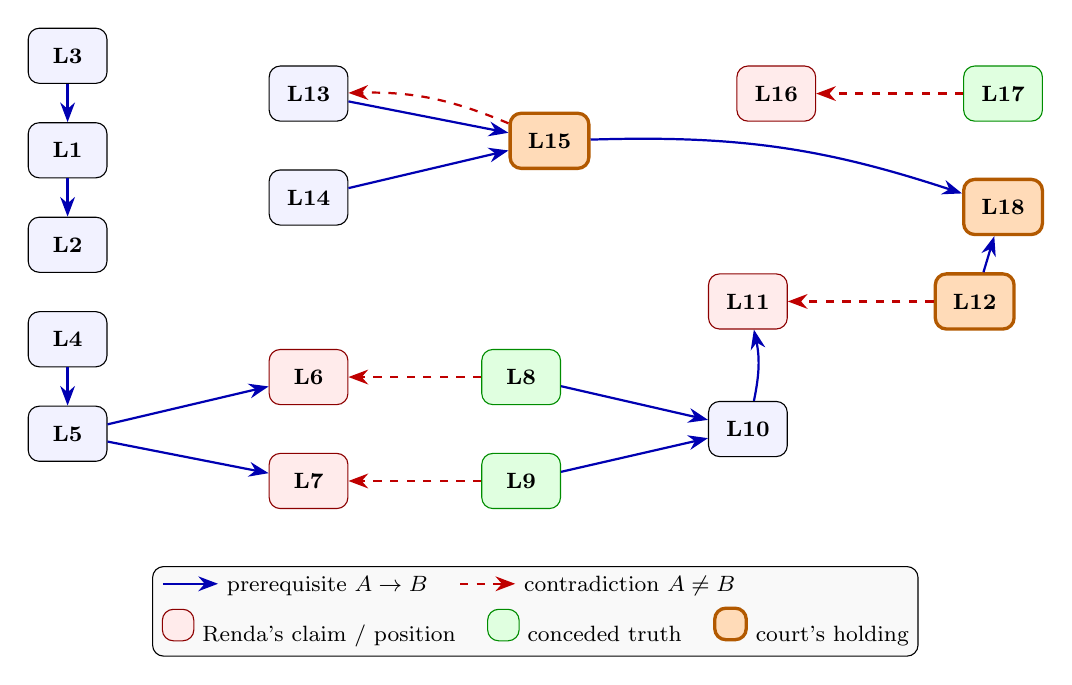
\begin{tikzpicture}[
    >={Stealth[length=2.5mm]},
    x=18mm, y=12mm,
    lnode/.style={draw,rounded corners,minimum width=10mm,minimum height=7mm,
                  inner sep=1pt,font=\footnotesize\bfseries,fill=blue!5},
    claim/.style={lnode,fill=red!8,draw=red!55!black},
    truth/.style={lnode,fill=green!12,draw=green!55!black},
    hold/.style={lnode,fill=orange!28,draw=orange!70!black,very thick},
    prereq/.style={->,blue!70!black,thick},
    invalid/.style={->,red!75!black,dashed,thick},
  ]

  % --- prerequisite spine (left, vertical-ish): incident -> conviction -> appeal
  \node[lnode] (l3) at (0,4)   {L3};
  \node[lnode] (l1) at (0,3)   {L1};
  \node[lnode] (l2) at (0,2)   {L2};
  \node[lnode] (l4) at (0,1)   {L4};
  \node[lnode] (l5) at (0,0)   {L5};

  % --- credibility contradiction pairs (claims left-mid, truths right) ---
  \node[claim] (l6) at (1.7,0.6) {L6};
  \node[claim] (l7) at (1.7,-0.5) {L7};
  \node[truth] (l8) at (3.2,0.6) {L8};
  \node[truth] (l9) at (3.2,-0.5) {L9};
  \node[lnode] (l10) at (4.8,0.05) {L10};

  % --- withdrawal argument pair ---
  \node[claim] (l11) at (4.8,1.4) {L11};
  \node[hold]  (l12) at (6.4,1.4) {L12};

  % --- bad-character cluster (upper right) ---
  \node[lnode] (l13) at (1.7,3.6) {L13};
  \node[lnode] (l14) at (1.7,2.5) {L14};
  \node[hold]  (l15) at (3.4,3.1) {L15};

  % --- counsel reversal pair ---
  \node[claim] (l16) at (5.0,3.6) {L16};
  \node[truth] (l17) at (6.6,3.6) {L17};

  % --- disposition ---
  \node[hold]  (l18) at (6.6,2.4) {L18};

  % --- prerequisite edges ---
  \draw[prereq] (l3) -- (l1);
  \draw[prereq] (l1) -- (l2);
  \draw[prereq] (l4) -- (l5);
  \draw[prereq] (l5) -- (l6);
  \draw[prereq] (l5) -- (l7);
  \draw[prereq] (l8) -- (l10);
  \draw[prereq] (l9) -- (l10);
  \draw[prereq] (l10) to[bend right=12] (l11);
  \draw[prereq] (l13) -- (l15);
  \draw[prereq] (l14) -- (l15);
  % the dismissal L18 follows from the holdings that defeated the challenges
  \draw[prereq] (l12) -- (l18);
  \draw[prereq] (l15) to[bend left=10] (l18);

  % --- contradiction edges ---
  \draw[invalid] (l8) -- (l6);
  \draw[invalid] (l9) -- (l7);
  \draw[invalid] (l12) -- (l11);
  \draw[invalid] (l17) -- (l16);
  \draw[invalid] (l15) to[bend right=12] (l13);

  % --- legend ---
  \node[draw,fill=gray!5,rounded corners,anchor=north,align=left,
        font=\footnotesize] at (3.3,-1.4) {
    \tikz\draw[prereq](0,0)--(7mm,0);~prerequisite $A\rightarrow B$
    \quad
    \tikz\draw[invalid](0,0)--(7mm,0);~contradiction $A\neq B$\\[3pt]
    \tikz\node[claim,minimum width=4mm,minimum height=4mm]{};~Renda's claim / position
    \quad
    \tikz\node[truth,minimum width=4mm,minimum height=4mm]{};~conceded truth
    \quad
    \tikz\node[hold,minimum width=4mm,minimum height=4mm]{};~court's holding
  };

\end{tikzpicture}
\end{center}

\noindent\emph{(For legibility, purely sequential narration links among the
spine atoms L2--L5 and the bracketing of L16/L17 within the contamination
argument are summarised rather than drawn edge-by-edge.)}

\subsection*{A faithful, naturally-ordered summary K}

The summary S above was deliberately ordered (claims first, conceded truths
afterward) to manufacture positional contradictions. For contrast we now give a
\emph{faithful} summary \textbf{K} of the same Renda appeal that follows the
judgment's own logical and chronological order: each disputed claim is reported
\emph{together with} its resolution, and the court's reasoning is presented in
the sequence the court itself adopts. Under this ordering the relation structure
is almost entirely \emph{logical implication}; the only residual tensions are the
two points the court expressly adjudicates, and even these read as holdings that
\emph{resolve} an issue rather than as a later atom flatly contradicting an
earlier one.

\noindent\textbf{Plain text.}
\begin{quote}
Raymond Renda was convicted of attempted robbery before HHJ Van Der Werff and a
jury, and appealed. The charge arose when, at about 2~am on 10~November 2003, he
accosted Robert Flint on Mile End Road, followed him home, and seized him by the
neck while demanding money; because the only real question was whether any
offence had been committed, the trial turned on the relative credibility of Flint
and Renda. Seeking to present himself as a man of positive good character, Renda
testified that his serious head injury had been sustained on duty in the armed
forces and that he was in regular employment as a security guard; in truth,
however, the injury was sustained on holiday in a car accident and the security
work had been only short-term, so that this evidence conveyed a false impression
within s\,105(1). When Renda conceded these matters under cross-examination, the
court held that a concession extracted in cross-examination does not amount to a
withdrawal of the false impression under s\,105(3). To help correct that false
impression, the Crown was permitted to put a July~2001 incident before the jury:
Renda had then been found unfit to plead to assault and given an absolute
discharge, so he was not convicted, yet a jury had found as a fact that he struck
a man from behind with a wooden table leg, and the court held that this act was
reprehensible behaviour within the bad-character provisions notwithstanding the
absence of a conviction. A submission that the resulting evidence was
contaminated under s\,107 was rejected, the court holding that it was not
contaminated, and the appeal was dismissed.
\end{quote}

\noindent\textbf{Annotated.} Each clause is one atomic unit
\textsuperscript{\textbf{\scriptsize K\textit{n}}}. The faithful ordering folds
each disputed claim into its finding, so there are no contradiction colours here:
blue~=~neutral fact, orange~=~court's holding.

\begin{quote}
\fu{cFact}{Raymond Renda was convicted of attempted robbery before HHJ Van Der Werff and a jury, and appealed}{K1}. The charge arose when,
\fu{cFact}{at about 2~am on 10~November 2003, he accosted Robert Flint on Mile End Road, followed him home, and seized him by the neck while demanding money}{K2}; because the only real question was whether any offence had been committed,
\fu{cFact}{the trial turned on the relative credibility of Flint and Renda}{K3}.
\fu{cFact}{Seeking to present himself as a man of positive good character, Renda testified}{K4}
\fu{cFact}{that his serious head injury had been sustained on duty in the armed forces and that he was in regular employment as a security guard}{K5}; in truth, however,
\fu{cFact}{the injury was sustained on holiday in a car accident and the security work had been only short-term, so that this evidence conveyed a false impression within \mbox{s\,105(1)}}{K6}.
\fu{cFact}{When Renda conceded these matters under cross-examination}{K7}, the
\fu{cHold}{court held that a concession extracted in cross-examination does not amount to a withdrawal of the false impression under \mbox{s\,105(3)}}{K8}. To help correct that false impression,
\fu{cFact}{the Crown was permitted to put a July~2001 incident before the jury}{K9}:
\fu{cFact}{Renda had then been found unfit to plead to assault and given an absolute discharge, so he was not convicted}{K10}, yet
\fu{cFact}{a jury had found as a fact that he struck a man from behind with a wooden table leg}{K11}, and the
\fu{cHold}{court held that this act was reprehensible behaviour within the bad-character provisions notwithstanding the absence of a conviction}{K12}.
\fu{cFact}{A submission that the resulting evidence was contaminated under \mbox{s\,107}}{K13} was rejected, the
\fu{cHold}{court holding that it was not contaminated, and the appeal was dismissed}{K14, K15}.
\end{quote}

\subsection*{Atomic units of K (self-contained, in order of appearance)}
\begin{enumerate}[label=\textbf{K\arabic*.},leftmargin=*]
  \item Raymond Renda was convicted of attempted robbery and appealed against the conviction.
  \item Renda accosted Robert Flint on Mile End Road at about 2~am on 10~November 2003, followed him home, and seized him by the neck while demanding money.
  \item The trial turned on the relative credibility of Robert Flint and Raymond Renda.
  \item Renda testified seeking to present himself as a man of positive good character.
  \item Renda testified that his head injury was sustained on duty in the armed forces and that he was in regular employment as a security guard.
  \item In truth Renda's injury was sustained on holiday in a car accident and his security work had been only short-term, so his evidence conveyed a false impression within s\,105(1).
  \item Renda conceded these matters under cross-examination.
  \item The court held that a concession extracted in cross-examination does not amount to a withdrawal of the false impression under s\,105(3).
  \item To help correct the false impression, the Crown was permitted to put a July~2001 incident before the jury.
  \item In the July~2001 incident Renda was found unfit to plead to assault and given an absolute discharge, so he was not convicted.
  \item A jury had found as a fact that Renda struck a man from behind with a wooden table leg.
  \item The court held that the table-leg act was reprehensible behaviour within the bad-character provisions, notwithstanding the absence of a conviction.
  \item A submission was made that the evidence was contaminated under s\,107.
  \item The court held that the evidence was not contaminated.
  \item The appeal was dismissed.
\end{enumerate}

\subsection*{Relations}

\textbf{Logical prerequisites ($A \rightarrow B$).}
\begin{itemize}[leftmargin=*]
  \item K2 $\rightarrow$ K1 --- the attempted-robbery incident grounds the conviction and the appeal.
  \item K1 $\rightarrow$ K3 --- the contested conviction is what makes credibility the trial issue.
  \item K3 $\rightarrow$ K4 --- credibility being decisive is why Renda testified to his good character.
  \item K4 $\rightarrow$ K5 --- the good-character case comprises the specific claims about injury and employment.
  \item K5 $\rightarrow$ K6 --- the claims are what the truth contradicts, yielding the ``false impression'' finding.
  \item K6 $\rightarrow$ K7 --- there must be a false assertion for Renda to concede it under cross-examination.
  \item K7 $\rightarrow$ K8 --- the cross-examination concession is the act the s\,105(3) holding rules upon.
  \item K6 $\rightarrow$ K9 --- the false impression is what the July~2001 material is admitted to correct.
  \item K10,\,K11 $\rightarrow$ K12 --- the unfit-to-plead finding and the found-fact assault ground the ``reprehensible behaviour'' holding.
  \item K9 $\rightarrow$ K13 --- admitting the bad-character material is the premise of the contamination submission.
  \item K13 $\rightarrow$ K14 --- the contamination submission is what the ``not contaminated'' holding answers.
  \item K8,\,K12,\,K14 $\rightarrow$ K15 --- the three holdings against Renda jointly ground the dismissal.
\end{itemize}

\noindent
\textbf{Contradictions / position invalidations ($A \neq B$).} Under the faithful
ordering there are \emph{no} positional invalidations between asserted atoms:
each claim (K5) is reported together with its correction (K6), so the truth does
not appear later as a contradicting atom but as part of the same finding. The two
genuine tensions in the case are stated as \emph{holdings that resolve} an issue,
not as contradictions:
\begin{itemize}[leftmargin=*]
  \item K8 settles the s\,105(3) question (a forced concession is not a withdrawal) --- presented as a ruling, with no competing asserted atom left standing.
  \item K12 settles the reprehensible-behaviour question (conduct can be reprehensible though it produced no conviction, K10) --- again a ruling rather than a flat contradiction.
\end{itemize}

\noindent
\textbf{Note.} Comparing K with S (the same facts, deliberately reordered)
illustrates the point: positional invalidation is a property of how a text is
\emph{arranged}, not only of the facts it contains. A faithful, logically ordered
summary of \emph{Renda} carries the case's full content as an implication chain
from the incident (K2) to the dismissal (K15), with the disputed points absorbed
into the findings rather than surfacing as contradictions.

\subsection*{Relation graph}

Solid blue arrows are logical prerequisites ($A \rightarrow B$). The court's three
operative holdings (K8, K12, K14) are highlighted; together they ground the
dismissal K15. There are no contradiction edges --- the faithful ordering folds
each disputed claim into its finding. Nodes are placed on an explicit grid so no
edge crosses a node.

\begin{center}
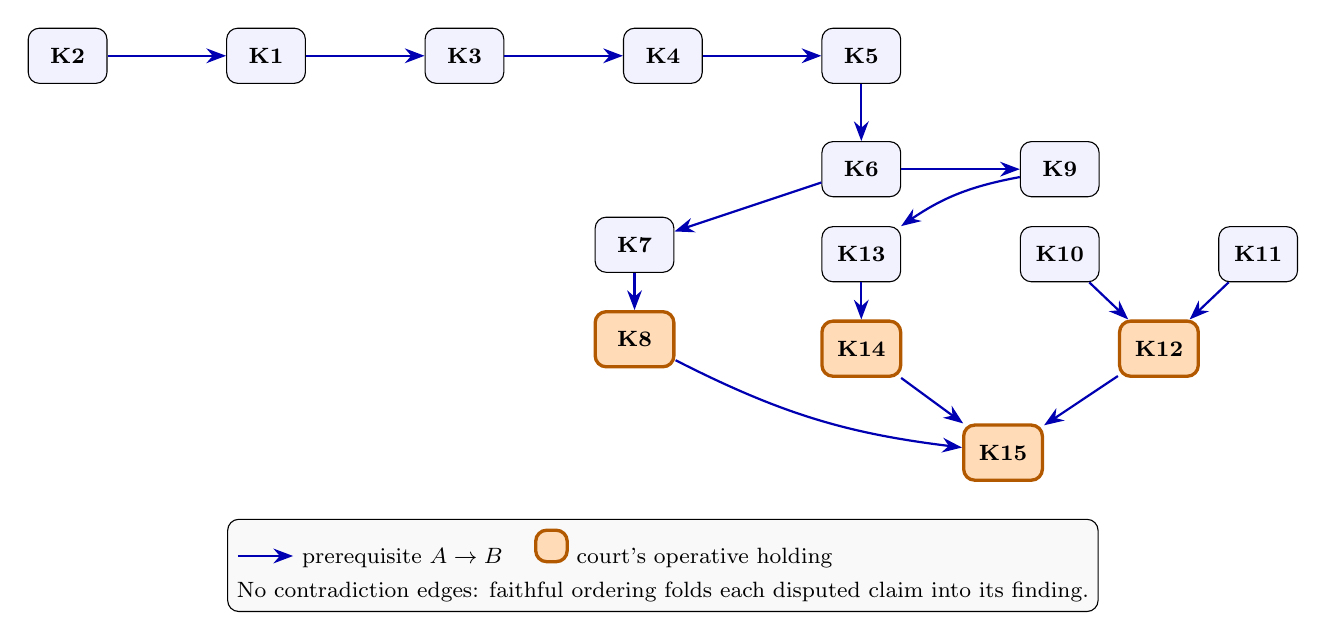
\begin{tikzpicture}[
    >={Stealth[length=2.5mm]},
    x=18mm, y=12mm,
    knode/.style={draw,rounded corners,minimum width=10mm,minimum height=7mm,
                  inner sep=1pt,font=\footnotesize\bfseries,fill=blue!5},
    hold/.style={knode,fill=orange!28,draw=orange!70!black,very thick},
    prereq/.style={->,blue!70!black,thick},
  ]

  % --- main spine (incident -> credibility -> good character -> claims) ---
  \node[knode] (k2) at (0,3)   {K2};
  \node[knode] (k1) at (1.4,3) {K1};
  \node[knode] (k3) at (2.8,3) {K3};
  \node[knode] (k4) at (4.2,3) {K4};
  \node[knode] (k5) at (5.6,3) {K5};

  % --- false impression and its two downstream branches ---
  \node[knode] (k6) at (5.6,1.8) {K6};

  % withdrawal branch (left-down)
  \node[knode] (k7) at (4.0,1.0) {K7};
  \node[hold]  (k8) at (4.0,0.0) {K8};

  % bad-character / correction branch (right-down)
  \node[knode] (k9)  at (7.0,1.8) {K9};
  \node[knode] (k10) at (7.0,0.9) {K10};
  \node[knode] (k11) at (8.4,0.9) {K11};
  \node[hold]  (k12) at (7.7,-0.1) {K12};
  \node[knode] (k13) at (5.6,0.9) {K13};
  \node[hold]  (k14) at (5.6,-0.1) {K14};

  % --- disposition ---
  \node[hold]  (k15) at (6.6,-1.2) {K15};

  % --- prerequisite edges ---
  \draw[prereq] (k2) -- (k1);
  \draw[prereq] (k1) -- (k3);
  \draw[prereq] (k3) -- (k4);
  \draw[prereq] (k4) -- (k5);
  \draw[prereq] (k5) -- (k6);
  \draw[prereq] (k6) -- (k7);
  \draw[prereq] (k7) -- (k8);
  \draw[prereq] (k6) -- (k9);
  \draw[prereq] (k10) -- (k12);
  \draw[prereq] (k11) -- (k12);
  \draw[prereq] (k9) to[bend right=12] (k13);
  \draw[prereq] (k13) -- (k14);
  \draw[prereq] (k8)  to[bend right=10] (k15);
  \draw[prereq] (k12) -- (k15);
  \draw[prereq] (k14) -- (k15);

  % --- legend ---
  \node[draw,fill=gray!5,rounded corners,anchor=north,align=left,
        font=\footnotesize] at (4.2,-1.9) {
    \tikz\draw[prereq](0,0)--(7mm,0);~prerequisite $A\rightarrow B$
    \quad
    \tikz\node[hold,minimum width=4mm,minimum height=4mm]{};~court's operative holding\\[3pt]
    No contradiction edges: faithful ordering folds each disputed claim into its finding.
  };

\end{tikzpicture}
\end{center}

\end{document}
